%%%% ijcai20.tex

\typeout{IJCAI--PRICAI--20 Instructions for Authors}

% These are the instructions for authors for IJCAI-20.

\documentclass{article}
\pdfpagewidth=8.5in
\pdfpageheight=11in
% The file ijcai20.sty is NOT the same than previous years'
\usepackage{ijcai20}

% Use the postscript times font!
\usepackage{times}
\usepackage{soul}
\usepackage{url}
\usepackage[hidelinks]{hyperref}
\usepackage[utf8]{inputenc}
\usepackage[small]{caption}
\usepackage{graphicx}
\usepackage{amsmath}
\usepackage{amsthm}
\usepackage{booktabs}
\usepackage{algorithm}
\usepackage{algorithmic}
\usepackage{listings}
\usepackage{hyperref}
\urlstyle{same}

% the following package is optional:
%\usepackage{latexsym} 

% See https://www.overleaf.com/learn/latex/theorems_and_proofs
% for a nice explanation of how to define new theorems, but keep
% in mind that the amsthm package is already included in this
% template and that you must *not* alter the styling.
\newtheorem{example}{Example}
\newtheorem{theorem}{Theorem}

% Following comment is from ijcai97-submit.tex:
% The preparation of these files was supported by Schlumberger Palo Alto
% Research, AT\&T Bell Laboratories, and Morgan Kaufmann Publishers.
% Shirley Jowell, of Morgan Kaufmann Publishers, and Peter F.
% Patel-Schneider, of AT\&T Bell Laboratories collaborated on their
% preparation.

% These instructions can be modified and used in other conferences as long
% as credit to the authors and supporting agencies is retained, this notice
% is not changed, and further modification or reuse is not restricted.
% Neither Shirley Jowell nor Peter F. Patel-Schneider can be listed as
% contacts for providing assistance without their prior permission.

% To use for other conferences, change references to files and the
% conference appropriate and use other authors, contacts, publishers, and
% organizations.
% Also change the deadline and address for returning papers and the length and
% page charge instructions.
% Put where the files are available in the appropriate places.

\title{Federated Meta Learning}

% Check the ijcai20-multiauthor.tex file for detailed instructions

\author{
Mukesh Arambakam$^1$
\and
Joeran Beel$^2$
\affiliations
$^1$Trinity College Dublin,
School of Computer Science and Statistics\\
$^2$Trinity College Dublin,
School of Computer Science and Statistics,
Artificial Intelligence Discipline,
ADAPT Centre
\emails
\{arambakm, beelj\}@tcd.ie
}


\begin{document}

\maketitle

\begin{abstract}
“Federated Meta-Learning” (FML), a concept that allows everyone to benefit from the data that is generated through software libraries including machine learning and data science libraries. We have built COOL-TOOL-NAME to achieve this, an application that allows the exchange of meta-data about machine learning models for the purpose of meta-learned algorithm selection and configuration across disciplines.
COOL-TOOL-NAME and scikit-learn's toy datasets were used and evaluated against various machine learning algorithms for which the execution time was measured. In the case of scikit-learn’s breast cancer dataset, it resulted in the execution time of 0.039sec and 0.596sec for SVC and GradientBoostingClassifier respectively along with 8 other algorithms to identify the algorithm with best performance (least MSE). Use of COOL-TOOL-NAME to identify the best algorithm for a dataset allows the user in scaling down the repetitive effort and time consumed in rewriting and executing code, correcting possible human errors, etc.
\end{abstract}

\section{Overview and Related Work}
There are an ever-growing number of algorithms used to solve machine learning and data science tasks and the challenge of algorithm selection and configuration is subject to intensive research. \cite{bischl-et-al,brazdil:p,calandra-et-al,collins-et-al2018,cunha-et-al2017,edenhofer-et-al,ferrari-et-al,hutter-et-al,kotthoff:l,lindauer-et-al,romero-et-al,tu:w,vartak-et-al}.

Meta-learning is one of the most promising techniques to warm starting the algorithm selection and configuration process \cite{hutter-et-al}. With meta-learning, a machine learning model is trained to predict how algorithms perform on a given task. The meta-learning model is built based on the past performance of algorithms on a large number of tasks (datasets), which are described through meta-features, and for new unseen tasks, the most performant algorithms can be predicted through the meta-learner.

A challenge in algorithm selection and configuration is the (non) availability of data in some disciplines to build the meta-learning model. This is due to the typical workflow of machine learning, data science, etc. Typically, software libraries – be it machine learning libraries like (Auto) sklearn, or recommender system libraries like LibRec (-Auto) are used in isolation, either locally or in the cloud. Either way, the information about how different the algorithms and their configurations perform on a particular dataset, is neither published nor shared with others.

The goal is to facilitate the algorithm selection process by leveraging historic performance data that was on various devices by various software libraries to improve the performance of algorithm and save time in finding the best algorithm for a task.


\section{COOL-TOOL-NAME}
Here we would like to introduce the concept called “Federated Meta-Learning” (FML), To the best of our knowledge this concept is novel. The term “Federated Meta Learning” has only been used once before by Chen et al. but in a different context \cite{chen-et-al}. 

Federated Meta Learning has similarities with “federated machine learning”, which was recently introduced by Google: “Federated [Machine] Learning enables [devices] to collaboratively learn a shared prediction model while keeping all the training data on device, decoupling the ability to do machine learning from the need to store the data in the cloud.”1 However, Federated Machine Learning focuses on learning one machine learning task across multiple devices. Whereas, Federated Meta Learning focuses on learning algorithm performance for arbitrary tasks across devices. We envision federated meta learning as an ecosystem where the raw data is kept on the original devices when the meta data would be stored in a central device. 

“COOL-TOOL-NAME” has been developed to implement this concept, it is a tool that allows everyone to benefit from the data that is generated through software libraries including machine learning and data science libraries as well as the auto* tools and tools from other domains. COOL-TOOL-NAME has a client-server architecture that allows the exchange of meta-data and performance metrics for the purpose of meta-learned algorithm selection and configuration across disciplines, and the machine-learning library scikit-learn has also been modified to make API calls to COOL-TOOL-NAME so as to perform the above mentioned operations. This knowledge base is built and updated by users who use COOL-TOOL-NAME by sending meta-data of their model’s and dataset’s  via scikit-learn to COOL-TOOL-NAME.

\url{https://github.com/mukeshmk/fml-back-end}

The input to COOL-TOOL-NAME is a hashed dataset of the task, and the output is a recommendation for the potentially best performing algorithm(s) to solve that task (see Figure 1). This recommendation consists either of a list of the best algorithms or simply the best performing algorithm and their predicted performance values. In its simplest form, COOL-TOOL-NAME is a knowledge base or directory of algorithms-data performance measures.

\begin{figure}[ht]
    \centering
    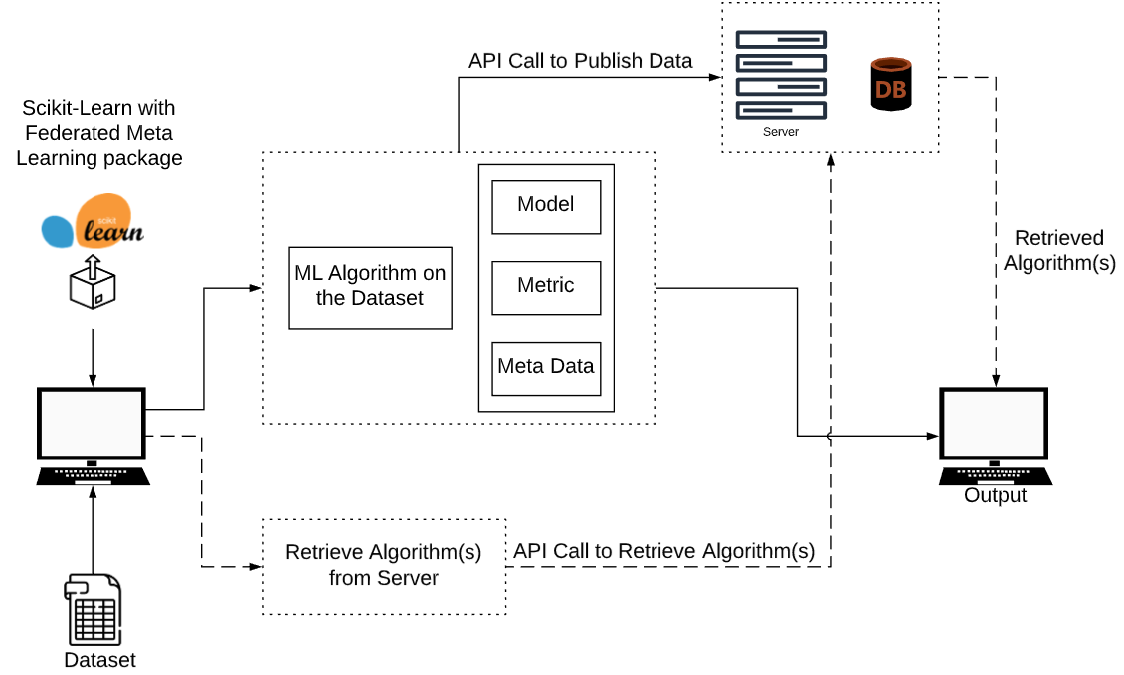
\includegraphics[width=3.5in]{architecture-diagram.PNG}
    \caption{Architecture Diagram}
    \label{architecture-diagram}
\end{figure}

Scikit-learn Internally makes the following API call to publish the data sent by the user to the server.
\begin{lstlisting}
POST: /metric
data-params: 
{model, name, value, hashed-dataset}
\end{lstlisting}

These API calls are used to retrieve all, the best algorithm with minimum metric value, and the best algorithm with maximum metric value respectively from the server given a hashed-dataset as a data parameter to the API calls.
\begin{lstlisting}
POST: /metric/retrieve/all
data-params: {hashed-dataset}
POST: /metric/retrieve/min
data-params: {hashed-dataset}
POST: /metric/retrieve/max
data-params: {hashed-dataset}
\end{lstlisting}

These API's are exposed via scikit-learn library by importing the following package and by making appropriate function calls:
\begin{lstlisting}[language=python]
from sklearn.fml import FMLClient
\end{lstlisting}

A sample of the output for an API call via scikit-learn for one of it's toy data-sets (Breast Cancer Wisconsin (diagnostic) dataset) \cite{william-et-al} is as follows (see figure 2):
\begin{lstlisting}[language=python]
f.retrieve_best_metric(data_set, True)
\end{lstlisting}
\begin{figure}[ht]
    \centering
    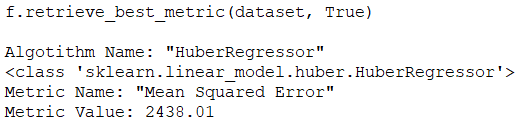
\includegraphics[width=3.5in]{sample-output.PNG}
    \caption{Sample Output}
    \label{sample-output}
\end{figure}


\section{Evaluation}
COOL-TOOL-NAME and scikit-learn's toy datasets were used and evaluated against various machine learning algorithms for which the execution time was measured. In the case of scikit-learn’s Breast Cancer Wisconsin (diagnostic) dataset \cite{william-et-al}, execution time of 0.039sec and 0.596sec were recorded for SVC and GradientBoostingClassifier respectively, execution time of 8 other algorithms were also measured to identify the algorithm with best performance over the given dataset (algorithm with least MSE). The algorithm with the best metric was HuberRegressor with an MSE of 2438.005. Use of COOL-TOOL-NAME to identify the best performing algorithm for a given dataset allows the user in scaling down the repetitive effort and time consumed in rewriting and executing code, correcting possible human errors, etc.

\section{Limitations and Future Work}
Currently COOL-TOOL-NAME only suggests algorithm(s), if the hashed dataset provided as the input is an exact match to that in the database, if an exact match is not found the user is notified that `there isn’t any algorithm recommendation for the given dataset`. So, a generic data description language is to be introduced to the system which is powerful enough to handle requests from data from various disciplines. The database only stores values like algorithm name, metric name, metric value and the hash dataset, there is scope  future implementation, which is to store even more meta data about the model like the model parameters and metrics for various configurations. In the long run, social questions need consideration such as preventing manipulation (developers of algorithms may have an interest that their algorithms are `recommended`) and free-rider problems (users benefiting from the system without sharing their data). Another challenge would arise if the system should not only focus on the globally best algorithm for a task (an entire dataset) but if per-instance algorithm selection should be learned. Ultimately, COOL-TOOL-NAME should be able to predict algorithm performance for unseen tasks. This would make the whole system even more complex.

\begin{thebibliography}{9}
\bibitem{bischl-et-al}
Bischl, B., Kerschke, P., Kotthoff, L., Lindauer, M., Malitsky, Y., Fréchette, A., Hoos, H., Hutter, F., Leyton-Brown, K., Tierney, K. and others 2016. Aslib: A benchmark library for algorithm selection. Artificial Intelligence. 237, (2016), 41–58.

\bibitem{brazdil:p}
Brazdil, P. 2014. Metalearning \& Algorithm Selection. 21st European Conference on Artificial Intelligence (ECAI). (2014).

\bibitem{calandra-et-al}
Calandra, R., Hutter, F., Larochelle, H. and Levine, S. 2017. Workshop on Meta-Learning (MetaLearn 2017) @NIPS. http://metalearning.ml (2017).

\bibitem{chen-et-al}
Chen, F., Dong, Z., Li, Z. and He, X. 2018. Federated Meta-Learning for Recommendation. arXiv preprint arXiv:1802.07876. (2018).

\bibitem{collins-et-al2018}
Collins, A., Tkaczyk, D. and Beel, J. 2018. A Novel Approach to Recommendation Algorithm Selection using Meta-Learning. Proceedings of the 26th Irish Conference on Artificial Intelligence and Cognitive Science (AICS) (2018), 210–219.

\bibitem{cunha-et-al2017}
Cunha, T., Soares, C. and Carvalho, A.C. 2017. Metalearning for Context-aware Filtering: Selection of Tensor Factorization Algorithms. Proceedings of the Eleventh ACM Conference on Recommender Systems (2017), 14–22.

\bibitem{edenhofer-et-al}
Edenhofer, G., Collins, A., Aizawa, A. and Beel, J. 2019. Augmenting the DonorsChoose.org Corpus for Meta-Learning. Proceedings of The 1st Interdisciplinary Workshop on Algorithm Selection and Meta-Learning in Information Retrieval (AMIR) (2019), 32–38.

\bibitem{ferrari-et-al}
Ferrari, D.G. and De Castro, L.N. 2015. Clustering algorithm selection by meta-learning systems: A new distance-based problem characterization and ranking combination methods. Information Sciences. 301, (2015), 181–194.

\bibitem{hutter-et-al}
Hutter, F., Kotthoff, L. and Vanschoren, J. 2019. Automatic machine learning: methods, systems, challenges. Challenges in Machine Learning. (2019).

\bibitem{kotthoff:l}
Kotthoff, L. 2016. Algorithm selection for combinatorial search problems: A survey. Data Mining and Constraint Programming. Springer. 149–190.

\bibitem{lindauer-et-al}
Lindauer, M., Rijn, J.N. van and Kotthoff, L. 2018. The Algorithm Selection Competition Series 2015-17. arXiv preprint arXiv:1805.01214. (2018).

\bibitem{romero-et-al}
Romero, C., Olmo, J.L. and Ventura, S. 2013. A meta-learning approach for recommending a subset of white-box classification algorithms for Moodle datasets. Educational Data Mining 2013 (2013).

\bibitem{tu:w}
Tu, W.-W. 2018. The 3rd AutoML Challenge: AutoML for Lifelong Machine Learning. NIPS 2018 Challenge (2018).

\bibitem{vartak-et-al}
Vartak, M., Thiagarajan, A., Miranda, C., Bratman, J. and Larochelle, H. 2017. A Meta-Learning Perspective on Cold-Start Recommendations for Items. Advances in Neural Information Processing Systems (2017), 6907–6917.

\bibitem{xu-et-al}
Xu, L., Hutter, F., Hoos, H.H. and Leyton-Brown, K. 2008. SATzilla: portfolio-based algorithm selection for SAT. Journal of artificial intelligence research. 32, (2008), 565–606.

\bibitem{william-et-al}
William H Wolberg, W Nick Street, and Olvi L Mangasarian. 1992. Breast cancer Wisconsin (diagnostic) data set. UCI Machine Learning Repository {http://archive.ics.uci.edu/ml/} (1992)

\end{thebibliography}

%% The file named.bst is a bibliography style file for BibTeX 0.99c
\bibliographystyle{named}
\bibliography{ijcai20}

\end{document}

